\documentclass[12pt]{article}
\setlength{\oddsidemargin}{0in}
\setlength{\evensidemargin}{0in}
\setlength{\textwidth}{6.5in}
\setlength{\parindent}{0in}
\setlength{\parskip}{\baselineskip}
\usepackage{amsmath,amsfonts,amssymb}
\usepackage{graphicx}
\usepackage[]{algorithmicx}
\usepackage{enumitem}
\usepackage{fancyvrb}
\usepackage{ wasysym }
\usepackage{tkz-berge}
\usetikzlibrary{positioning, automata}
\usepackage{algpseudocode}

\usepackage{fancyhdr}
\pagestyle{fancy}
\setlength{\headsep}{36pt}

\usepackage{hyperref}


\hypersetup{
	colorlinks=true,
	linkcolor=blue,
	filecolor=magenta,      
	urlcolor=blue,
}

\newcommand{\makenonemptybox}[2]{%
	%\par\nobreak\vspace{\ht\strutbox}\noindent
	\item[]
	\fbox{% added -2\fboxrule to specified width to avoid overfull hboxes
		% and removed the -2\fboxsep from height specification (image not updated)
		% because in MWE 2cm is should be height of contents excluding sep and frame
		\parbox[c][#1][t]{\dimexpr\linewidth-2\fboxsep-2\fboxrule}{
			\hrule width \hsize height 0pt
			#2
		}%
	}%
	\par\vspace{\ht\strutbox}
}
\makeatother

\begin{document}
	\lhead{{\bf CSCI 3104, Algorithms \\ Homework 5A (40 points)} }
	\rhead{Name: \fbox{% Place your name here and delete the next time
			\phantom{This is a really long name}} 
		\\ ID: \fbox{ % Place your ID here and delete the next time
			\phantom{This is a student ID}} 
		\\ {\bf Escobedo \& Jahagirdar\\ Summer 2020, CU-Boulder}}
	\renewcommand{\headrulewidth}{0.5pt}
	
	\phantom{Test}
	
	\begin{small}
		\textit{Advice 1}:\ For every problem in this class, you must justify your answer:\ show how you arrived at it and why it is correct. If there are assumptions you need to make along the way, state those clearly.
		%\vspace{-3mm} 
		
		\textit{Advice 2}:\ Verbal reasoning is typically insufficient for full credit. Instead, write a logical argument, in the style of a mathematical proof.\\
		%\vspace{-3mm} 
		
		\textbf{Instructions for submitting your solution}:
		\vspace{-5mm} 
		
		\begin{itemize}
			\item The solutions \textbf{should be typed}, we cannot accept hand-written solutions. Here's a short intro to \href{http://ece.uprm.edu/~caceros/latex/introduction.pdf}{\textbf{Latex}.}
			\item In this homework we denote the asymptomatic \textit{Big-O} notation by $\mathcal{O}$ and \textit{Small-O} notation is represented as $o$. 
			\item We recommend using online Latex editor \href{https://www.overleaf.com/}{\textbf{Overleaf}}. Download the \textbf{.tex} file from Canvas and upload it on overleaf to edit.
			%todo add link of gradescope
			\item You should submit your work through \href{https://www.gradescope.com}{\textbf{Gradescope}}  only.
			\item If you don't have an account on it, sign up for one using your CU email. You should have gotten an email to sign up. If your name based CU email doesn't work, try the identikey@colorado.edu version. 
			\item Gradescope will only accept \textbf{.pdf} files (except for code files that should be submitted separately on Canvas if a problem set has them) and \textbf{try to fit your work in the box provided}. 
			\item You cannot submit a pdf which has less pages than what we provided you as Gradescope won't allow it.
			
		\end{itemize}
		\vspace{-4mm} 
	\end{small}
	
	\hrulefill
	\pagebreak
	
	\subsection*{Piazza threads for hints and further discussion}
	\begin{center}
		\begin{tabular}{|c|}
			\hline
			Piazza Threads \\ [0.5ex] 
			\hline \hline 
			\href{https://piazza.com/class/ka2roz7rb9m3j4?cid=75}{Question 1}\\
			\href{https://piazza.com/class/ka2roz7rb9m3j4?cid=76}{Question 2}\\
			\href{https://piazza.com/class/ka2roz7rb9m3j4?cid=77}{Question 3}\\
			\href{https://piazza.com/class/ka2roz7rb9m3j4?cid=78}{Question 4}\\
			\hline
		\end{tabular}
	\end{center}
	
	\textbf{Recommended reading}: \\
	Graph Algorithms Intro: Ch. 22 $\to$ 22.1, 22.2, 22.3 \\
	Graph Algorithms SSSPs: Ch. 24 $\to$ 24.3
	\\
	
	\pagebreak
	
	\begin{enumerate}
		
		\item
		(5 pts) Consider the following unweighted directed graph.
		\begin{figure}[h!]
			\begin{center}
				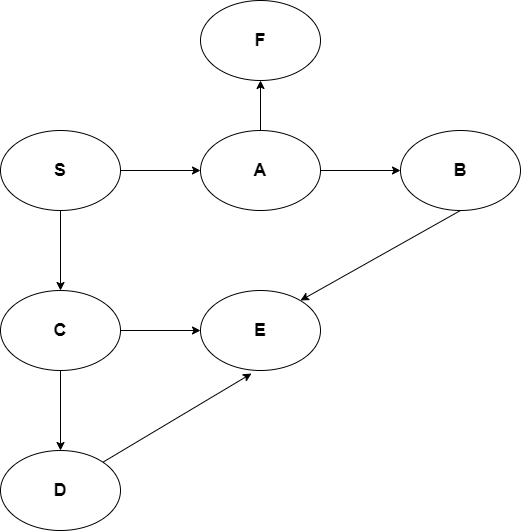
\includegraphics[scale=0.5]{/home/satyam/1593781628-hw5/hw5/graph_question.png}
			\end{center}
		\end{figure}
		\begin{enumerate}
			\item 
			(2.5 pts) Write down the order in which nodes are visited if Depth First Search (DFS) is called on the above graph with \textbf{S} as the source node.\\
			\makenonemptybox{2.5in}{There can be many possible DFS for the above graph. Such possible DFS are 1.S,A,F,B,E,C,D \\2. S,C,D,E,A,F,B\\3.S,A,B,E,F,C,D\\4.S,C,D,E,A,F,B\\5.S,C,E,D,A,B,F}
			
			\item 
			(2.5 pts) Write down the order in which nodes are visited if Breadth First Search (BFS) is called on the above graph with \textbf{S} as the source node.\\
			\makenonemptybox{3in}{Ordering of BFS are :1. S, A, C,F,B,D,E\\2. S, C, A, D, E, F,B\\3.S,C,A,E,D,B,F\\4.S,A,C,B,F,D,E}
		\end{enumerate}
		\clearpage
		%----------------------------------------------------------------------------------------------
		\item (5 pts)
		A simple path $s \to t$  in a graph $G$ is a path starting at $s$, ending at $t$, and
		never visiting the same vertex twice. Give an example graph (simple, undirected,
		unweighted) $G = (V;E)$ and vertices $s, t \in  V$ such that DFS finds a path from $s$ to $t$
		which is neither a shortest path nor a longest simple path. Detail the execution of DFS
		(list the contents of the stack at each step, and which vertex it pops off the stack),
		show the final $s \to t$ path it finds, show a shorter $s \to t$ path, and a longer simple
		$s \to t$ path.
		\makenonemptybox{5in}{Assume complete graph $K_{4}$,where every vertices are having weight of 1. The nodes are numbered 1,2,3,4 and assume source is at node 1 and destination is at node 3. \\Execution details of $K_{4}$: Initially stack is empty. Since 1 is the source node,it is pushed into stack.\\
		\textbf{Stack Status: 1}\\It has 2 choices either 2 or 4. Assume 2 is visited.\textbf{Stack Status: 1,2 }\\It has 2 choices either to choose node 3 or node 4. Assume 3 is visited, which is also destination. \textbf{Stack Status: 1,2,3 }

			
			
			\\Shortest path will be from 1-3, \\Longest path will be either 1,2,4,3 or 1,4,2,3,\\ Final path : 1-2-3 or 1-4-3.}
		\clearpage
		%----------------------------------------------------------------------------------------------
		\item 
		(20 pts) Assume you're given an integer matrix that representing islands in an ocean. A value of 0 in a particular cell indicates water and a value of 1 indicated land. An island is region of land connected vertically, horizontally, or diagonally.  The size of an island is the total number of connected land cells. Write an algorithm to compute the sizes of all islands in the matrix. Example:
		\begin{verbatim}
		1 0 0 1
		0 1 0 1
		0 1 0 0
		0 1 0 1
		\end{verbatim}
		would output 1, 2, 4.
		\begin{enumerate}
			\item (6 pts) State if the graph data structure that your algorithm will use for this problem will be i) be weighted or unweighted and ii) directed or undirected. In addition, iii) what makes two nodes have an edge/connection? Give an explanation for each of your answers. 
			
			\makenonemptybox{4in}{The graph will be (i)unweighted, as the adjacency matrix doesn't have values other than 0 or 1.\\ (ii) directed, as the required output is one of the possibility.It is possible, only when the graph is directed. Assume $I_{i}$, $\forall i \in {1,2,3,4}$ is represented by Nodes 1,2,3,4. The nodes 1 have outgoing edge, 2 and 4 has bidirectional edges.\\(iii) 1 in the adjacency matrix represents the island and edges between the island and the both are connected.0 represents the water and it is not connected to any other island}
			\clearpage
			
			\item (4 pts) Provide a 3-4 sentence description of how your algorithm works, including how the matrix is converted to the graph, how adjacent vertices are identified, and how the algorithm traverses the graph to identify connected vertices.
			\makenonemptybox{3in}{ The 1's in the adjacency matrix  represents island,which are connected with another island and O's represents the island,which are not connnected.
		Assume $I_{i}$, $\forall i \in {1,2,3,4}$ is represented by Nodes 1,2,3,4. The node 1 have outgoing edge, node 2 and 4 has bidirectional edges and node 3 is not connected to any other island. Node 3 will be one component and Node 1,2,4 will be another component. The algorithm uses Depth-First Search (DFS) on the connected components.
			
		}
			\clearpage
			
			\item (10 pts) Write well commented pseudo or real code to solve this problem. 
			\makenonemptybox{8in}{Pseudo code will consists of 3 procedure(or function). Procedure DFS will be used to find the  order of the connected components of adjacent neighbours. Procedure Visited : To check if the given row,col must be included in the DFS and not yet visited. Procedure print: The order of connected components. 
			
		\begin{algorithmic}[1]
		
		\Statex
		\State $ROW \gets 4$
		\State $COL \gets 4$
		\Function{visited}{M[][COL],r,bool visited[][COL]}
		\Comment{row number is in range, column number is in range and value is 1 \\ and not yet visited }
		\State \Return $(row \geq 0) and (row < ROW) and (col \geq 0) and (col < COL) $
		\EndFunction
		
		\Function{DFS}{M[][COL],r,c,bool visited[][COL]}
		\Comment{Function of DFS,which will consider  8 adjacent neighbours}
		\State Array $rowNbr = \{-1, -1, -1, 0, 0, 1, 1, 1\}$
		\Comment{These arrays are used to get 
row and column numbers of 8 
neighbours of a given cell }
		\State Array $colNbr = \{ -1, 0, 1, -1, 1, -1, 0, 1 \}$ 
		\State Array $visited[r][c]\gets true$
		\Comment{Mark this cell as visited }
		\State \For{$k \gets 0$ to $k<8$}{\State \If{{\Call {Visited}{M, r + rowNbr[k], c+ colNbr[k], visited}}} 

			{{\Call {DFS}{M, r + rowNbr[k], c + colNbr[k], visited}}
}
	\EndIf	} 
		\EndFor
\EndFunction
		
		\Function{print}{M[][COL])}
		\Comment{To print the order of island }
		\State $visited[ROW][COL]$
		\newpage
		\State \For{$i \gets 0$ to $ROW$}{
		{\State \For{$j \gets 0$ to $COL$}{
	%	\Comment{Traverse the row and col and check if the node is visited or not.\\ If not visited visit that node and include in the list}
		\State \If{M[i][j] and visited[i][j]==False}
			\Call{DFS}{M, i, j, visited}	
	\EndIf
	}
\\print Order
\EndFor}\EndFor}\EndFunction
		
	\end{algorithmic}	
	}
			\clearpage
		\end{enumerate}
		
		
		\item (10 pts) Using Dijkstra's algorithm, determine the length of the shortest path from $v_{0}$ to each of the other vertices in the graph. Clearly specify the distances from $v_{0}$ to each vertex \textbf{after each iteration} of the algorithm.
		
		\begin{center}
			\begin {tikzpicture}[-latex ,auto ,node distance =2 cm and 3cm ,on grid ,
			semithick ,
			state/.style ={ circle ,top color =white , bottom color = processblue!20 ,
				draw,processblue , text=blue , minimum width =1 cm}]
			
			\node[state] (A) {$v_{0}$};
			\node[state] (B) [above right = of A] {$v_{1}$};
			\node[state] (C) [below right = of A] {$v_{2}$};
			\node[state] (D) [right = of B] {$v_{3}$};
			\node[state] (E) [right = of C] {$v_{4}$};
			\node[state] (F) [below right = of D] {$v_{5}$};
			\path (A) edge node[above] {$1$} (B);
			\path (A) edge node[right] {$5$} (C);
			\path (B) edge node[right] {$6$} (C);
			\path (B) edge node[above] {$2$} (D);
			\path (B) edge node[right] {$12$} (E);
			\path (C) edge node[above] {$4$} (E);
			\path (E) edge node[right] {$9$} (D);
			\path (D) edge node[above] {$12$} (F);
			\path (E) edge node[above] {$21$} (F);
			
			\path (C) edge [bend right = 50] node[below] {$3$} (F);
			
		\end{tikzpicture}  
	\end{center}
	
	\makenonemptybox{4in}{
		
		Shortest path from $v_{0}$ to every node is represented in the form of table
		\begin{center}

			\begin{tabular}{ |c|c|c|c|c| }

				\hline
				$v_{1}$ &$v_{2}$&$v_{3}$&$v_{4}$&$v_{5}$\\
				\hline
				1 & 5 & 3 & 9 & 8  
				\\ \hline  

			\end{tabular}

	\end{center}
\vspace{0.5cm} Initially all the vertices are having distance $\infty$. Source is initialized, which will have distance 0.\\$1^{st} $iteration, two choices so each adjacent vertices distance are updated as $min(1,\infty)$ for $v_{1}$ and $min(5,\infty)$ for $v_{2}$.Remaining vertices are $\infty$.\\
$2^{nd}$iteration, 3 path from $v_{1}$ are updated as $min(2,\infty)$ for $v_{3}$, $min(5,7)$ for $v_{2}$, $min(13,\infty)$ for $v_{4}$. $v_{5}$ still remains $\infty$\\
$3^{rd}$iteration, 2 path from $v_{2}$ are updated as $min(9,13)$ for $v_{4}$, $min(8,$\infty$)$  $v_{5}$.
$4^{th}$iteration, 2 path from $v_{4}$ are updated as $min(3,18)$ for $v_{3}$, $min(8,30)$  $v_{5}$.
}
	
	\item{\itshape \textbf{Extra Credit (5\% of total homework grade)}
		For this extra credit question, please refer the leetcode link provided below or click \href{https://leetcode.com/problems/keys-and-rooms/}{here}. Multiple solutions exist to this question ranging from brute force to the most optimal one. Points will be provided based on Time and Space Complexities relative to that of the most optimal solution.
		
		Please provide your solution with proper comments which carries points as well.}
	
	\url{https://leetcode.com/problems/keys-and-rooms/}
	
	% Paste your code in the verbatim tag below
	\begin{verbatim}
	Replace this text with your source code inside of the .tex document
	\end{verbatim}	
	
	
\end{enumerate}


\end{document}


